\documentclass[a4paper, 12pt]{article}
\usepackage{graphicx}
\usepackage{float}
\usepackage{booktabs}
\usepackage{tabularx}
\usepackage{sans}
\usepackage{caption}
\usepackage[list=true]{subcaption}
\usepackage{hyperref}
\usepackage{appendix}
\usepackage{siunitx}

\hypersetup{colorlinks=true, linkcolor=black}

\newcommand{\company}{CKR Consulting Engineers}

\begin{document}
	\hypersetup{pageanchor=false}
	\pagenumbering{gobble}
	\begin{titlepage}
		{\LARGE \centerline{Team Apex Shell Eco Marathon Funding Proposal}\par}
		\makebox[\textwidth][c]{
			
\includegraphics[width=\textwidth]{img/apex_logo.jpeg}
		}
		\vspace*{\fill}
		\makebox[\textwidth][c]{
			
\includegraphics[width=0.4\linewidth]{img/shell.png}\hspace*{\fill}
\includegraphics[width=0.4\linewidth]{img/uj.jpg}
		}
		{\large\centering Funding proposal for the development and construction of a prototype battery electric vehicle to successfully take part in the Shell Eco Marathon 2018\par}
		\vspace*{\fill}
		\makebox[\textwidth][c]{\par\today}
	\end{titlepage}

	\hypersetup{pageanchor=true}
	\pagenumbering{roman}
	\tableofcontents
	\listoffigures
	\newpage

	% Signatory page
	\section*{Signatory Page} % (fold)
	\label{sec:signatory_page}
		\vspace*{8em}
		\hspace*{1cm}
\includegraphics[width=0.2\textwidth]{img/prof_sig.png}\hspace*{\fill}
\includegraphics[width=0.2\textwidth]{img/prof_date.png}\vspace*{1em}\par\noindent
		\makebox[\textwidth][l]{Prof J. Meyer \hspace*{7cm} Date}
		{Head of School, Electrical Engineering\par}
		\vspace*{8em}
		\hspace*{1cm}
\includegraphics[width=0.14\textwidth]{img/wes_sig.png}\hspace*{\fill}
\includegraphics[width=0.2\textwidth]{img/wes_date.png}\vspace*{1em}\par\noindent
		\noindent\makebox[\textwidth][l]{Wesley Richardson \hspace*{6.2cm} Date}
		{Team Apex CEO}\par
		\vspace*{\fill}
		\noindent\textit{Please note that Professor Johan Meyer's signature only serves to prove that this event is legitimately one that the University of Johannesburg participates in, and does not show that he explicitly approves of the budget.}
	% section signatory_page (end)
	\newpage
	\pagenumbering{arabic}
	\section{Executive summary} % (fold)
	\label{sec:overview}
		We are Apex, a team of engineering students at the University of Johannesburg who are enrolled in the Systems Engineering \& Design module. As part of this module, we have to participate in the Shell Eco Marathon, taking place from 25 October to 28 October. Apex has to construct and prepare a vehicle that is driven by an electric motor, and participate in the race to see how efficient we can make it.
		\vspace*{\fill}
		\begin{figure}[H]
			\centering
			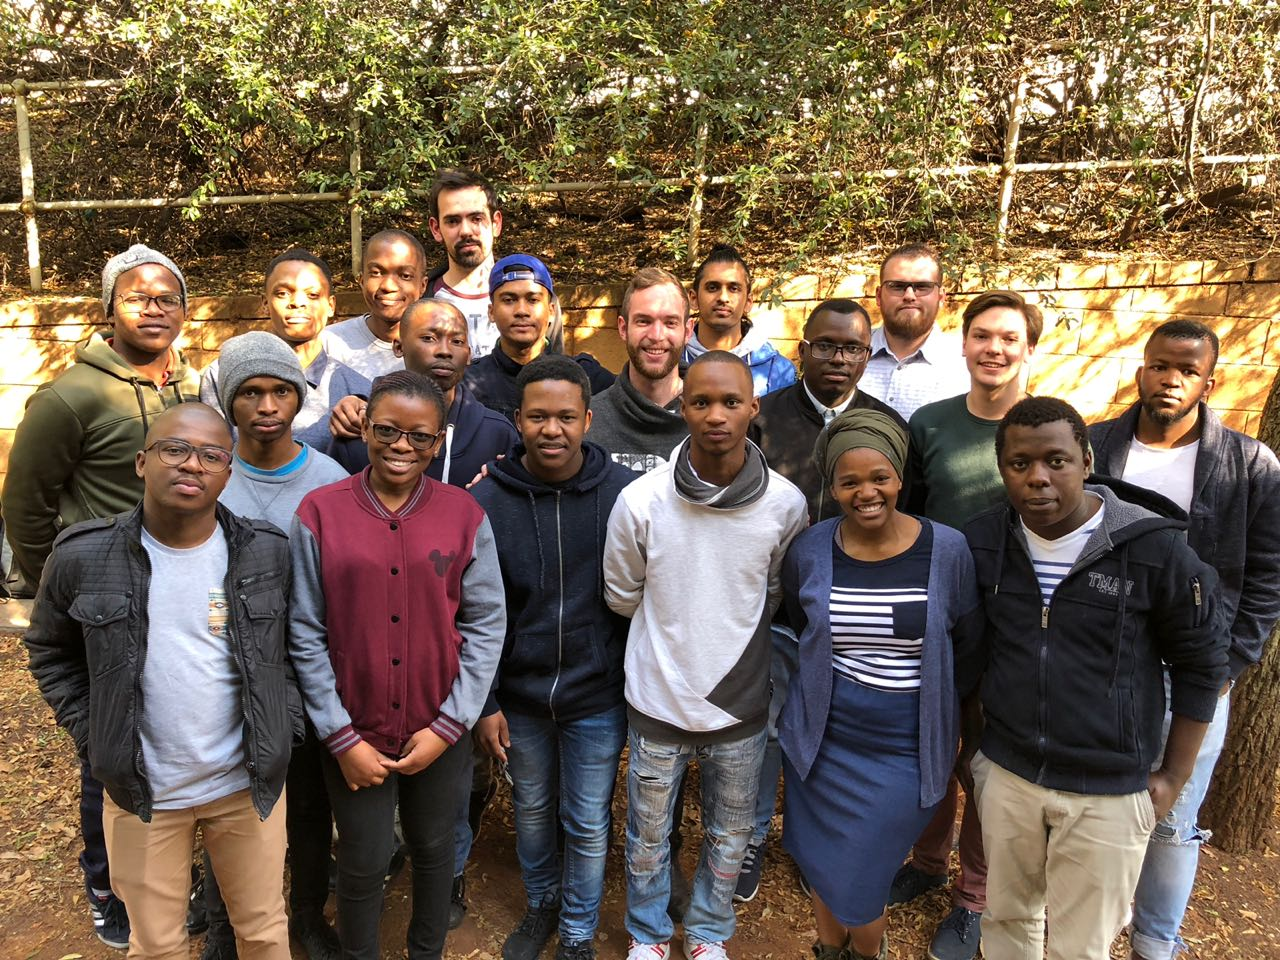
\includegraphics[width=0.7\textwidth]{img/group.jpg}
			\caption{Team Apex}
		\end{figure}

		\begin{figure}[H]
			% \centering
			\begin{subfigure}{0.5\textwidth}
				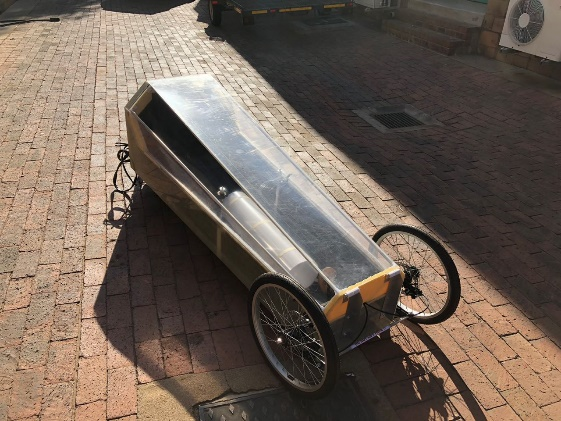
\includegraphics{img/front_view.jpg}
				\caption{Front view}
			\end{subfigure}
			\begin{subfigure}{0.5\textwidth}
				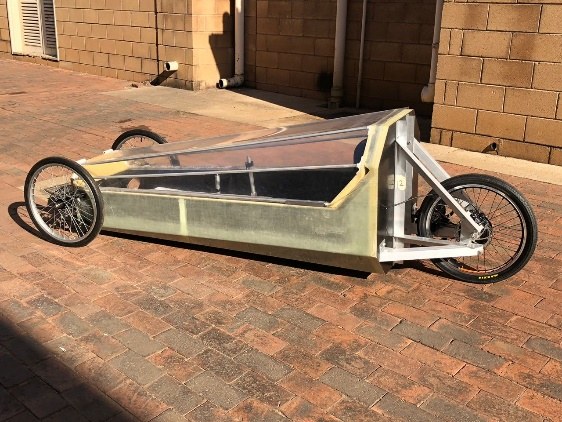
\includegraphics{img/side_view.jpg}
				\caption{Side view}
			\end{subfigure}
			\caption{Shell Eco Marathon vehicle}
		\end{figure}
	% section overview (end)
	\newpage
	\section{The Shell Eco Marathon} % (fold)
	\label{sec:the_shell_eco_marathon}
		The Shell Eco Marathon started out as a simple friendly bet between Shell scientists in the USA in 1939, who wanted to see who could drive their own cars the furthest on one gallon of fuel. Since then, this humble bet between friends and colleagues has become an institution. The Shell Eco Marathon is held all over the world, with nine events scheduled for 2018, including France, Turkey, China, South Africa. Teams compete in international events, and the best competitors get to compete in the Driver's World Championship.

		We as Apex are a group of engineering students from the University of Johannesburg. The group was created with the vision of designing and building a car for the Shell Eco-Marathon competition sponsored by the Shell Company. The main objective of this project is to design, build and test a battery-driven vehicle.

		The competition allows students and other competitors to impart their knowledge and turn their vision of sustainable mobility into reality by building automotive vehicles to achieve the highest possible battery electric efficiency. The competition is split into two categories, the prototype class and the urban concept class; we will be building the prototype cars, which focuses on maximum efficiency using a battery driven propulsion system. The efficiency of the vehicle will be determined at the end of the race day event.
	% section the_shell_eco_marathon (end)

	\section{Technical} % (fold)
	\label{sec:technical}
		\subsection{Measuring efficiency} % (fold)
		\label{sub:measuring_efficiency}
			The aim of the competition is to have the most efficient vehicle. During the event, all teams are allowed to make multiple race attempts. Each attempt consists of a few laps around the track. Each vehicle is given a maximum amount of time in order to complete the race, and at the end of these laps, the vehicle is measured for efficiency. In the case of the battery-driven prototype class, the efficiency is determined by placing a Joulemeter between the motor controller and the battery. At the end of the race, this provides an efficiency metric measured in km/kWh. The team with the highest efficiency by the end of the event wins.
		% subsection measuring_efficiency (end)

		\subsection{Telemetry} % (fold)
		\label{sub:telemetry_solution}
			The key assumption we make behind the efficiency of the vehicle, is that the slower it is driven, the more efficient it will be. We make this assumption, because the faster the vehicle drives, the larger the drag force that must be counteracted by the vehicle. With a larger drag force, also comes a larger downforce, which increases the effect of rolling friction from the wheels. At higher speeds, more power draw from the battery is required, and when going around turns, more energy is also expended by the deformation of the wheels. 

			With that in mind, our key tactic behind winning the race will be making sure that the vehicle drives as slowly as is permissible, and should finish the race just short of the maximum allowable time per race attempt. We aim to achieve this by using a Raspberry Pi, and a GPS module. The GPS module will gather positional data throughout the race, and the distance between this data can be calculated using the Haversine formula. We can use discrete differentiation between these points in order to calculate the velocity of the vehicle. We will then display the processed data on a screen inside the vehicle for the driver, which will display
			\begin{enumerate}
				\item Distance traveled
				\item Current lap
				\item Current speed
				\item Recommended speed
			\end{enumerate}

			The current lap and distance traveled are useful metrics for the driver to have, as during our research phase, we have spoken to teams who have competed in previous years, and they claim that an unforeseen problem that they have encountered was that the drivers get confused during the race, and are unsure which lap they are on or how far they have driven. This uncertainty distracts the driver and negatively affects their performance. Providing the driver with this information allows them to focus on the cornerstone of our system; the speed regulation mechanisms. By using the positional data, we can easily calculate how far the driver still needs to drive, as well as how much time is left for the race attempt. Using this, we will display the driver a recommended speed that they need to travel that dynamically changes throughout the race. The driver must then make sure that their current speed matches the recommended speed, and maintain this throughout the race in order to maximize efficiency.
		% subsection telemetry_solution (end)

		\subsection{Accuracy of GPS tracking} % (fold)
		\label{sub:accuracy_of_gps_tracking}
			The accuracy of the GPS coordinates are of utmost importance to ensure that accurate distance and speed can be derived from them. We plan to implement a Kalman Filter algorithm to enhance the accuracy of the GPS coordinates we track. This is fairly easy to achieve, as the errors in the GPS coordinates can be measured by letting the GPS unit be stationary, and logging several hundred samples for analysis. This will give us a credible and objective measure of error in GPS measurements. We will feed this error into the Kalman Filter to smooth out measurements and gain much more accurate estimations of instantaneous position. Furthermore, the velocity of the vehicle itself will also be tracked using the Kalman Filter, which will increase the accuracy of velocity estimation around bends.
		% subsection accuracy_of_gps_tracking (end)

		\subsection{Modifications}
		\label{sub:modifications}
			As part of the Shell Eco Marathon Chapter 1 Rules, the vehicle is required to have a crumple zone of at least $100mm$ between the front of the car and the driver's feet. The Apex team has thus decided to add a front and back modification to the vehicle (see the appendices \ref{sec:front_modification} and \ref{sec:back_modification} for the design). The rules have also stated that sharp edge designs are prohibited. Having this restriction, our modification design has rounded edges.

			Figure \ref{fig:front_view_dimensions} shows a green contour that represents the thickness of the shell to be attached to the front portion of the car that must be $40mm$ in width. Similarly Figure \ref{fig:back_view_dimensions} shows a similar contour with a similar thickness.

			The material that will be used to form the cones will be PETG plastic. This specific grade of plastic has been chosen as it is what the rest of the car has already been constructed with and is a plastic that offers good impact resistance. 
		% subsection modifications (end)
	% section technical (end)

	\section{Cost} % (fold)
	\label{sec:cost}
		Apex only has a ``bare bones'' vehicle to start off with, that simply has a body, three wheels, a few transparent PETG plastic panels, and a motor. We must bring the car to a state in which it is ready to race by the 25th of October. The following table outlines the budget to accomplish this.

		\begin{table}[H]
			\begin{tabularx}{\textwidth}{Xr}
				\toprule
				\textbf{Item} & \textbf{Cost} \\
				\midrule
				Driver's gear & 5\,200.00 \\
				Fire Extinguisher & 130.00 \\
				Safety harness & 3\,000.00 \\
				Rear view mirrors & 250.00 \\
				\addlinespace[0.7em]
				Electrical components and telemetry & 3\,500.00 \\
				Communication system & 700.00 \\
				Battery & 3\,300.00 \\
				Battery fire safety bag & 600.00 \\
				\addlinespace[0.7em]
				First Aid Kit & 600.00 \\
				Overhead & 4\,650.00 \\
				Contingency & 2\,600.00 \\
				\addlinespace[0.3em]
				\midrule
				\textbf{Total} & \textbf{R\,24\,530.00}\\
				\bottomrule
			\end{tabularx}
		\end{table}

		The battery is a single 48V unit that will be used to power the vehicle. The telemetry system will be used to track the coordinates of the vehicle in real time, and be used to provide the team and the driver with useful information like distance covered and current traveling speed, yielding the team greater control over the race. The safety equipment involves buying the driver a race suit, a 6-point safety harness, and a racing helmet.

		In addition to this, we must also equip the vehicle with brakes, emergency stops, and a horn. This will allow the driver to race around the track safely, and is of utmost importance. Management reserve refers to the weekend of the race itself. It is a four day event, from 25 October to 28 October, and the entire team of 19 people needs to be transported to and from Swartkopz Raceway, as well as being kept fed throughout the day while working on the vehicles.\\

		\noindent\textit{Note: we have, at the time of writing this proposal, not yet received a quotation from the transportation services we plan to use\footnote{Services are provided in the form of buses by the University of Johannesburg, although students and clubs of the university who wish to use it still need to provide payment.}. We have factored in an estimated cost while we wait for the quotation. If \company{} would like to provide us with alternatives regarding transportation, we would be open to such offers.}
	% section cost (end)

	\section{Benefits to \company{}} % (fold)
	\label{sec:benefits_to_the_client}
		\subsection{Marketing} % (fold)
		\label{sub:marketing}
			The Shell Eco Marathon is an international event, with races held in nine countries, with an even larger amount of countries attending these races from all over the world. Clearly, this presents many marketing opportunities for a discerning sponsor; the team who wins the race gets a chance to compete in the Shell Eco Marathon World Championship Grand Final hosted in London. Now, Team Apex are willing to display the \company{} logo on signs in our team's racing pits on the day, as well as on the vehicle itself. Therefore, any promotional videos or photos which are taken of our car will openly show your company's brand.
		% subsection marketing (end)
		
		\subsection{Exposure to future employees} % (fold)
		\label{sub:exposure_to_future_employees}
			It seems like there's always a shortage of engineers, regardless of where you are. This is even more true in South Africa, and engineers are always valued employees. By agreeing to sponsor us, you will see the members of Team Apex from a unique point of view. You will get to discern our work ethic, passion, drive, knowledge, teamwork, and technical skills/knowledge - all of the things that you would determine from an engineer during a job interview - during the course of this project. This exposes \company{} to the kind of future employees you would prefer to have. At the end of the project, after the race event is done, you can keep in contact with the promising students you have identified, and offer them work opportunities.
		% subsection exposure_to_future_employees (end)
		\subsection{Public relations} % (fold)
		\label{sub:public_relations}
			This event poses a huge public relations opportunity for \company{}. By being involved with a student team during this event, you get to drop the fa\c{c}ade of men and women in suits and ties, whose sole concern is the bottom line. You show onlookers that you are open to investing in the local talent pool of engineers, who will one day go on to either build up South Africa, or represent it abroad. You show that \company{} cares about the environment, and moreover, involvement in fun events like this come across favorably in the public eye.
		% subsection public_relations (end)
	
	\section{Conclusion} % (fold)
	\label{sec:conclusion}
		Team Apex is a group of dedicated and disciplined students, eager to succeed in this project. Apex has gone to great lengths to research the development of a custom telemetry and tracking solution using a Raspberry Pi and GPS module, that suits our goals and requirements, and will provide real time and logged race-relevant data to both the driver as well as the team in the race pits, for analysis during the event. We have carefully designed the circuitry in the vehicle, and are confident that our innovative attitude makes us a very strong competitor in this event.
	% section conclusion (end)	
	% section benefits_to_the_client (end)

	\newpage
	\begin{appendices}
		\section{Front Modifications}
		\label{sec:front_modification}

			\begin{figure}[H]
				\centering
				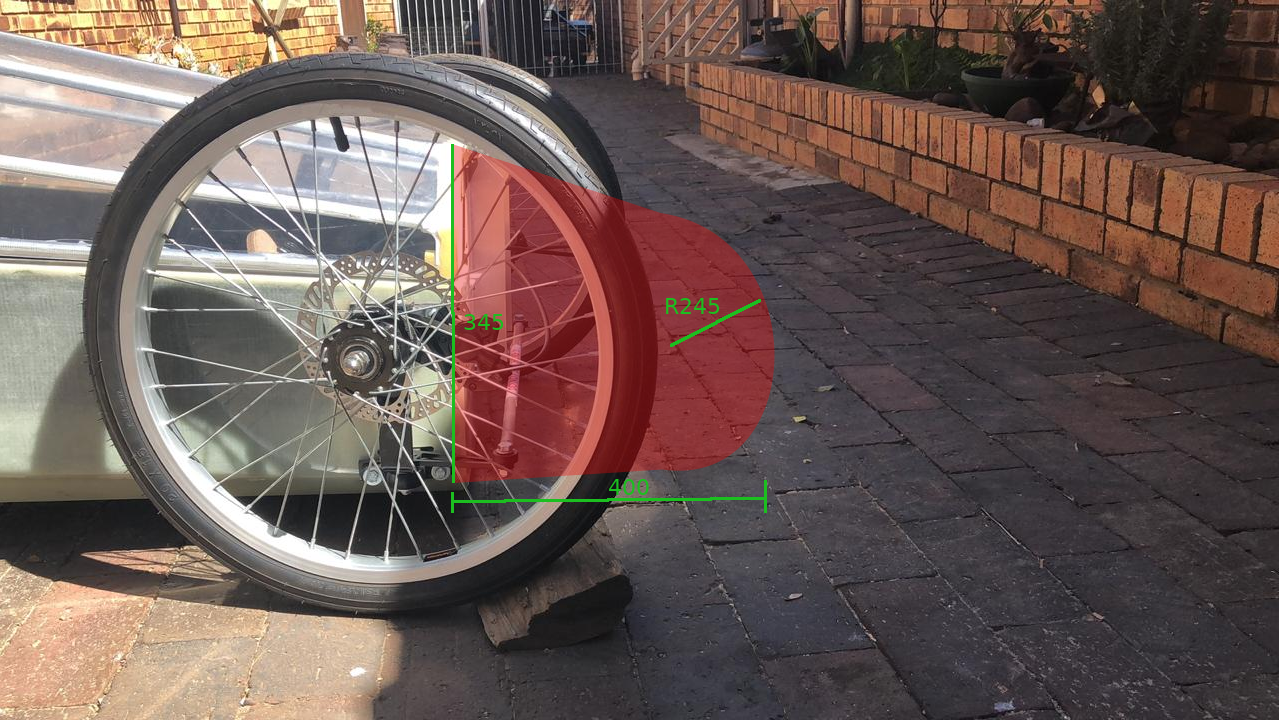
\includegraphics[width = 150mm]{img/Front_Side_View_Coned.png}
				\caption{Coned front view}
				\label{fig:front_side_view_coned}
			\end{figure}

			\begin{figure}[H]
				\centering
				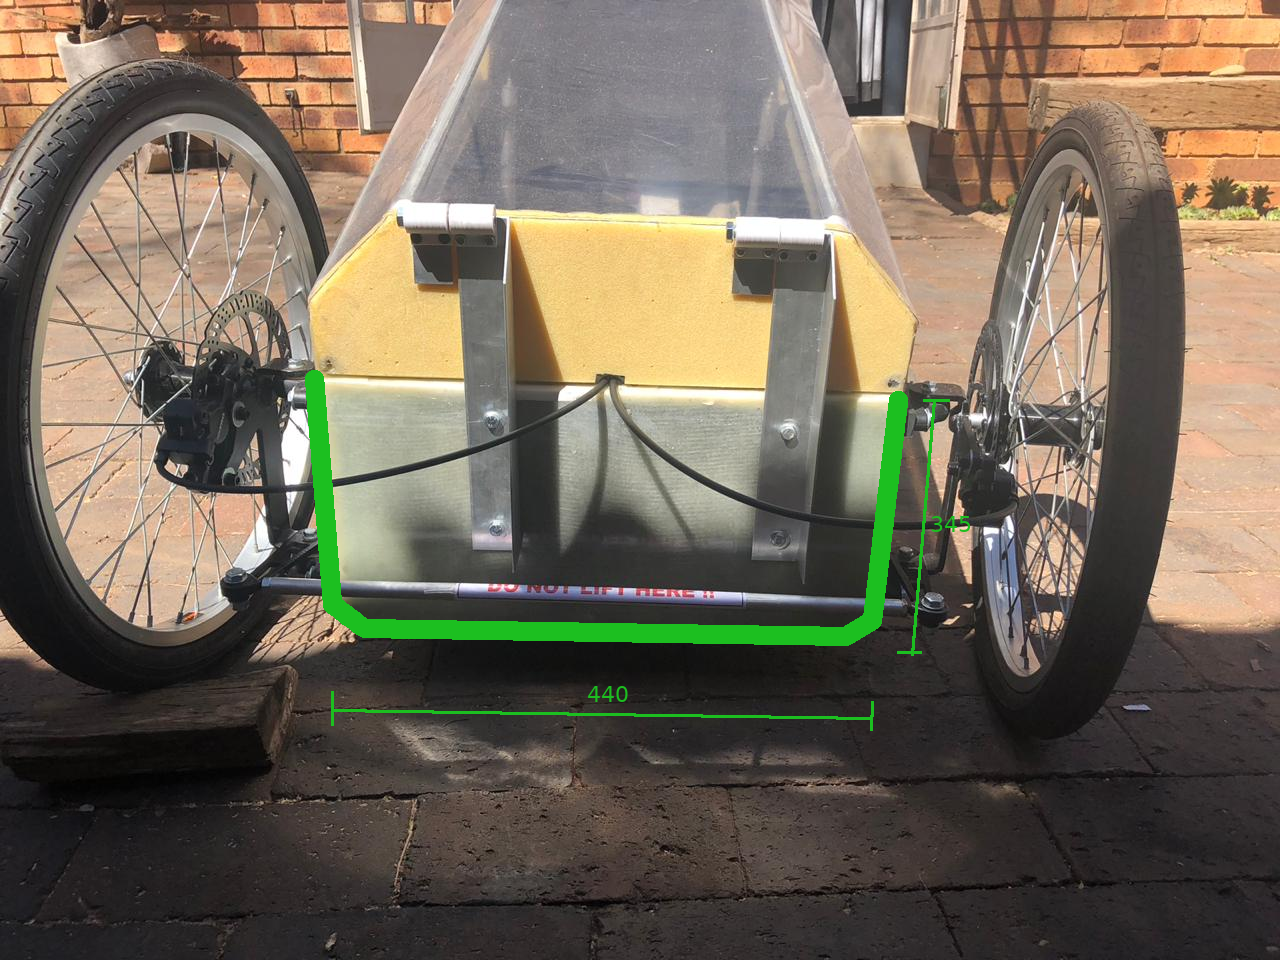
\includegraphics[width = 150mm]{img/Front_View_Dimensions.png}
				\caption{Side view}
				\label{fig:front_view_dimensions}
			\end{figure}

	

		\section{Back Modification}
		\label{sec:back_modification}

		\begin{figure}[H]
			\centering
			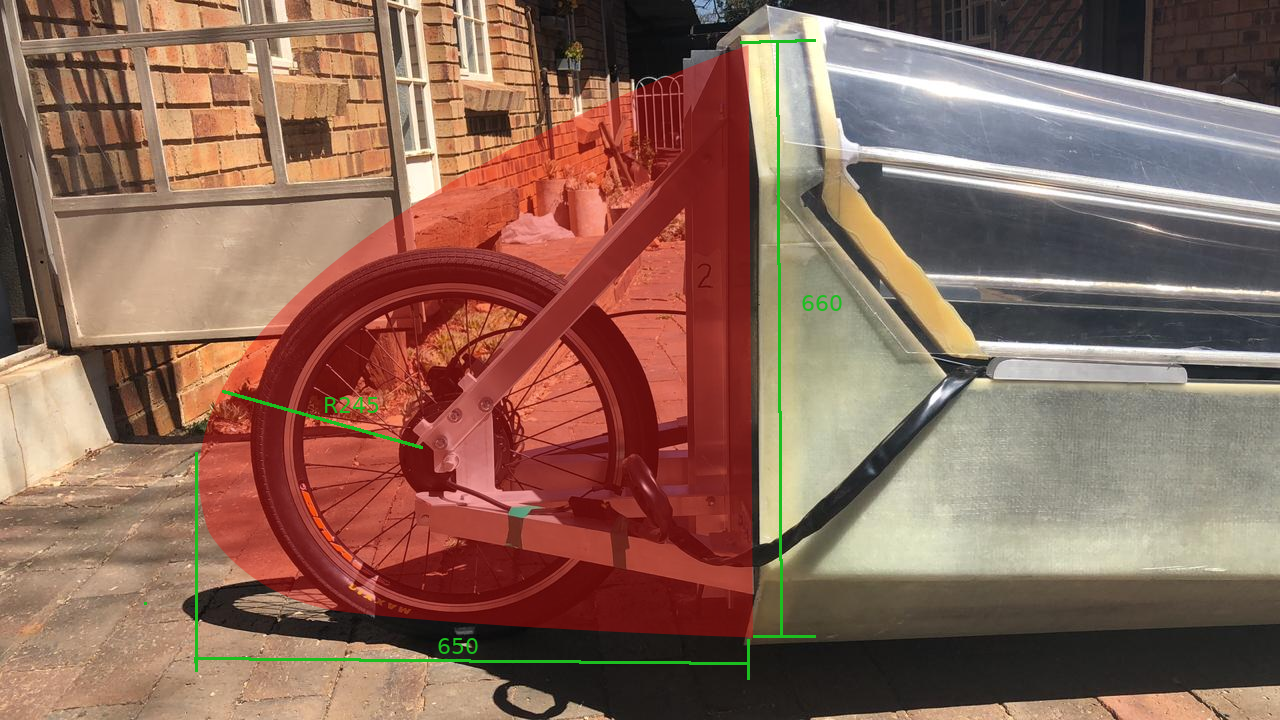
\includegraphics[width = 150mm]{img/Back_Side_View_Coned.png}
			\caption{Coned back view}
			\label{fig:coned_back_view}
		\end{figure}

		\begin{figure}[H]
			\centering
			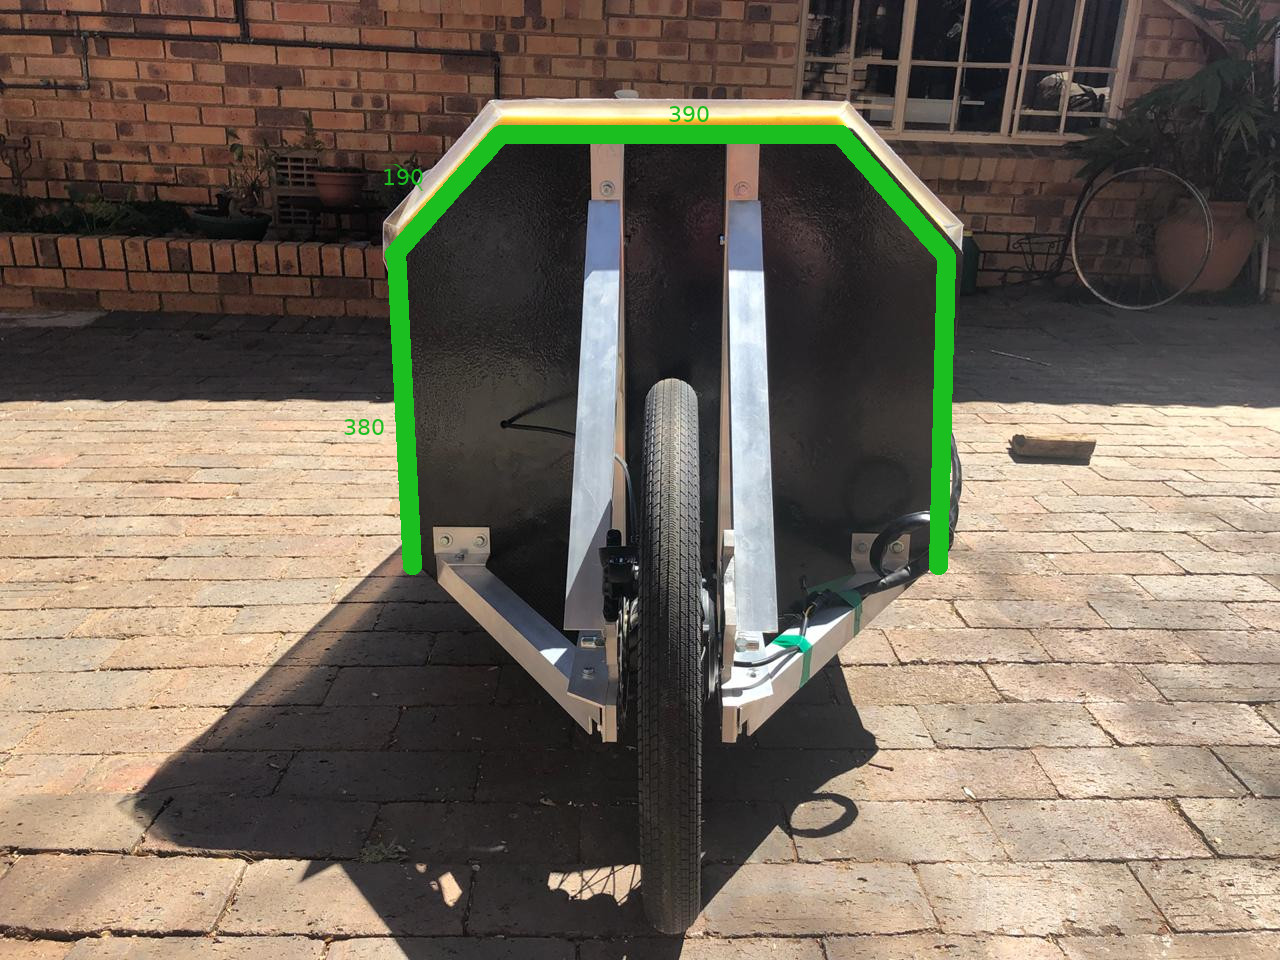
\includegraphics[width = 150mm]{img/Back_View_Dimensions.jpeg}
			\caption{Dimensions of cone}
			\label{fig:back_view_dimensions}
		\end{figure}

	\end{appendices}
\end{document}